\documentclass[a4paper,11pt]{article}
\usepackage[T2A]{fontenc}     
\usepackage[utf8]{inputenc}  
\usepackage{lmodern}  
\usepackage{amsmath}
\usepackage{amsfonts}
\usepackage{amssymb} 
\usepackage{listings}
\usepackage{lstcustom}
\usepackage{graphicx}
\usepackage{pstricks}
\usepackage{geometry} % Меняем поля страницы
\geometry{left=2cm}% левое поле
\geometry{right=1.5cm}% правое поле
\geometry{top=1cm}% верхнее поле
\geometry{bottom=2cm}% нижнее поле
\renewcommand\lstlistingname{Листинг}
\renewcommand\contentsname{Содержание}
\renewcommand\partname{ }
\renewcommand{\thepart}{\arabic{part}}


\definecolor{javared}{rgb}{0.6,0,0} % for strings

\definecolor{javagreen}{rgb}{0.25,0.5,0.35} % comments

\definecolor{javapurple}{rgb}{0.5,0,0.35} % keywords

\definecolor{javadocblue}{rgb}{0.25,0.35,0.75} % javadoc




\author{Архангельский Илья}


\begin{document}
\begin{titlepage}
	\begin{center}
		БЕЛОРУССКИЙ ГОСУДАРСТВЕННЫЙ УНИВЕРСИТЕТ \\
		ФАКУЛЬТЕТ ПРИКЛАДНОЙ МАТЕМАТИКИ И ИНФОРМАТИКИ
	\end{center}
	\vspace{10em}
	\begin{center}
		\LARGE {Лабораторная работа \\
		по вычислительным методам алгебры на тему:}
		\linebreak	 
		
    Определение наибольшего по модулю собственного значения матрицы
	\end{center}
	\vspace{3em}
	\begin{flushright}
	  
	
 	Выполнил: \\	Архангельский И.А. \\ 
 	
 	  \vspace{1em}
 	
 	  Проверил: \\ Кондратюк А.П. \\
 	
	\end{flushright}
	
	\vfill
	\begin{center}
		Минск, 2012
	\end{center}
\end{titlepage} 

\newpage
\part*{Входные и выходные данные.} 
\section*{Входные данные}
Входной файл в первой строке содержит число $n$ - размерность матрицы , следующие $n$ строк содержат матрицу $(A)$, где  
  $A$ - квадратная матрица. \\
Строка $n+2$ содержит начальный вектор $y_0$. \\
Строка $n+3$ содержит величину $\varepsilon$ - заданную точность.
\section*{Выходные данные}
На выход в stdout подается максимальное собственное значение матрицы $A$
\newpage
\part*{Блок-схема} 
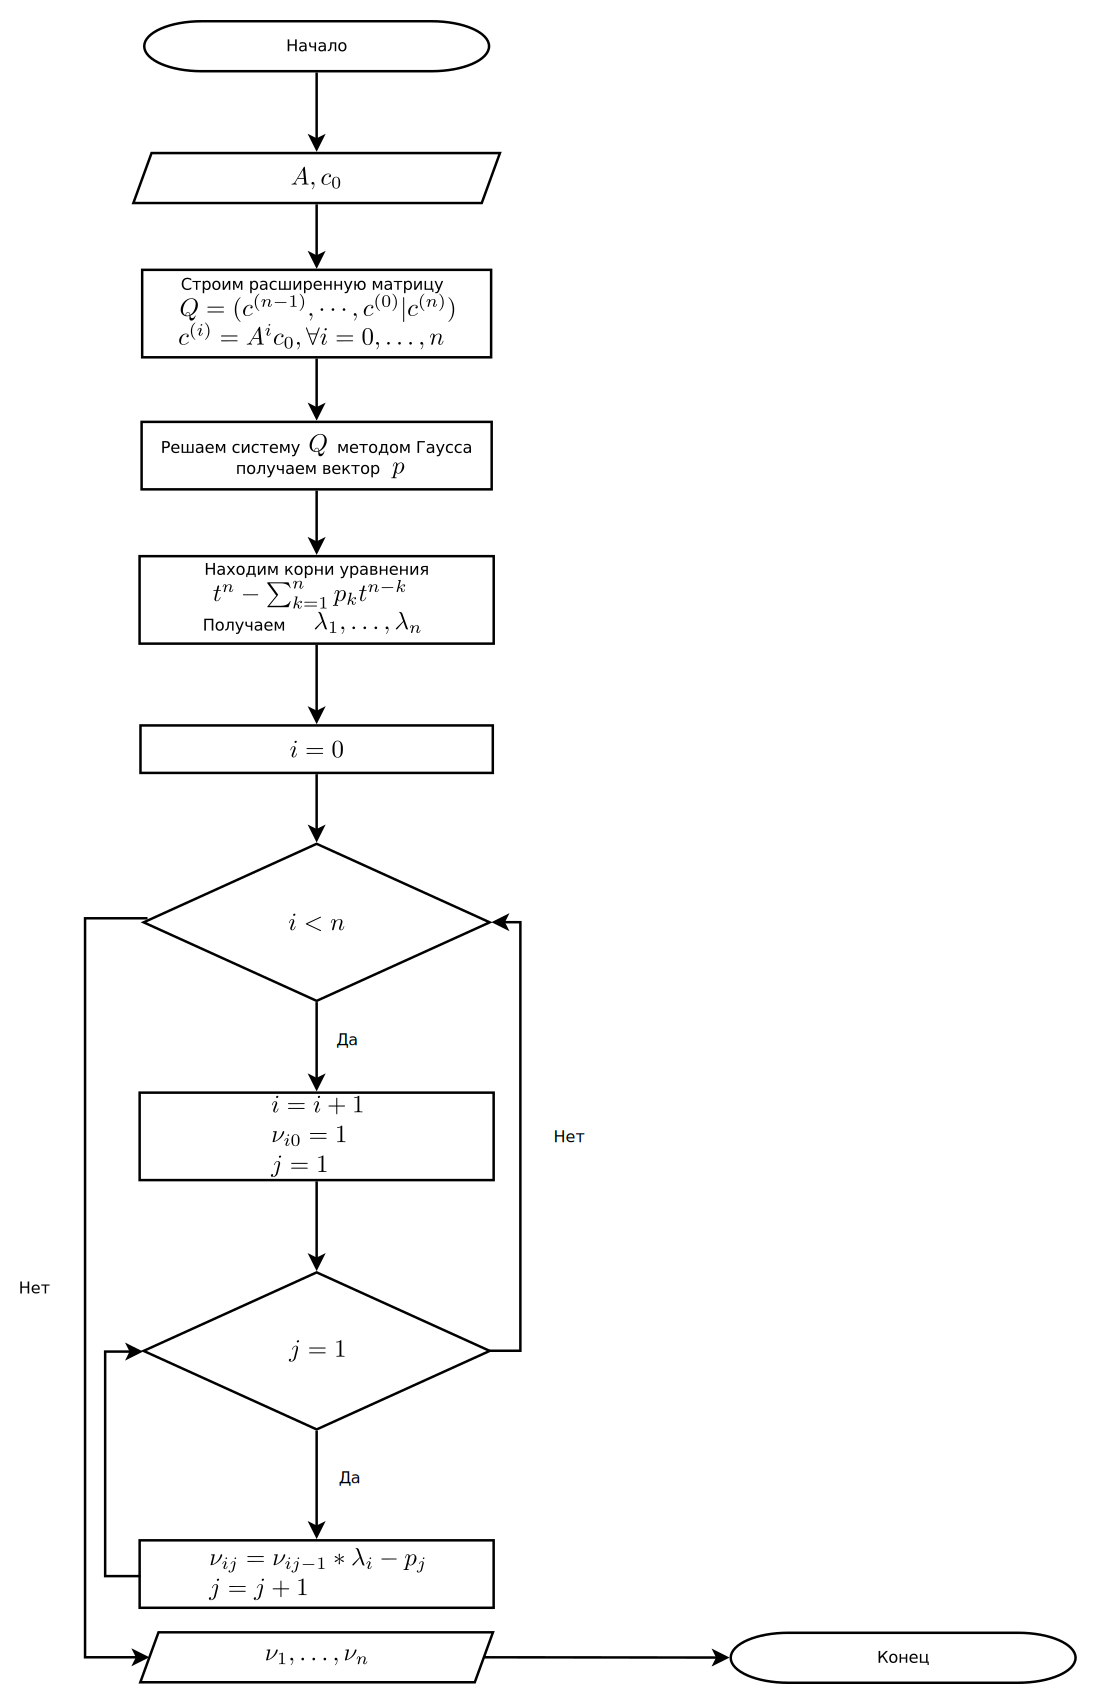
\includegraphics[scale=1]{flowchart.pdf}
 


\newpage
\part*{Реализация}


\lstinputlisting[language=Java,  style=eclipse, basicstyle=\scriptsize]{"../Maximum-Eigenvalue/src/maximumeigenvalue/MaximumEgien.java"}
 
 

 
 \newpage
\part*{Тестовые данные}
\begin{footnotesize}
\framebox{
  \begin{minipage}[t]{0.4\linewidth}   
  \lstinputlisting[title={test01.in}]{"../tests/test01.in"}
  \end{minipage}
  \begin{minipage}[t]{0.6\linewidth}
  \lstinputlisting[title={test01.out}]{"../tests/test01.out"}
  \end{minipage}
}
\framebox
{ 
  \begin{minipage}[t]{0.4\linewidth}   
  \lstinputlisting[title={test02.in}]{"../tests/test02.in"}
  \end{minipage}
  \begin{minipage}[t]{0.6\linewidth}
  \lstinputlisting[title={test02.out}]{"../tests/test02.out"}
  \end{minipage}
}
\framebox
{
  \begin{minipage}[t]{0.4\linewidth}
  \lstinputlisting[title={test03.in}]{"../tests/test03.in"}
  \end{minipage}
  \begin{minipage}[t]{0.6\linewidth}
  \lstinputlisting[title={test03.out}]{"../tests/test03.out"}
  \end{minipage}  
}
 
\end{footnotesize}
\end{document}
